\documentclass[12pt,a4paper]{article}
\usepackage{enumerate} 	% put in numbers or bullet points
\usepackage{setspace}	% line spacing					
\usepackage{authblk}	% For author affiliations
\usepackage{graphicx} 	% For adding pictures
\usepackage{pdflscape}	% for landscape pages
\usepackage{mathtools}	% For equations etc.
\usepackage[osf]{mathpazo} 
\usepackage{float}		
\floatstyle{plaintop} 	% Force table captions to go above the table
\usepackage{longtable}
\usepackage[margin ={2cm, 2cm, 2cm, 2cm}]{geometry}
\usepackage[round]{natbib}
%\setcounter{secnumdepth}{0} % removes numbers from section headings
\raggedright 			% justify the text on the left only
\pagenumbering{arabic}
\linespread{1.6}
	

\begin{document}

\title{
       Cranial morphological disparity within the adaptive radiation of tenrecs (Afrosoricida, Tenrecidae) is no greater than expected by chance\\
       \bigskip
       Supplementary Material }
\author{Sive Finlay and Natalie Cooper}
\date{}
\maketitle




%----------------------------------------------------
%Camera protocol
%---------------------------------------------------

\section{Photographing specimens}
One of us (SF) photographed the specimens with a Canon EOS 650D camera fitted with an EF 100mm f/2.8 Macro USM lens.We used a remote control (h\"ahnel Combi TF) to take the photos to avoid shaking the camera and distorting the images

We used photographic copy stands consisting of a camera attachment with an adjustable height bar, a flat stage on which to place the specimen and an adjustable light source to either side of the stage. We used the copy stands that were available at each museum which differed in how the camera height was adjusted and in the light sources available.
To take the light variability into account, on each day we took a picture of a white sheet of paper and used the custom white balance function on the camera to set the image as the baseline “white” measurement for those particular light conditions.

We photographed the specimens on a black material background with the light source in the top left-hand corner of the picture. We positioned a piece of white card on the bottom right side of the specimen to reflect the light back onto the specimen and therefore minimise any shadows (figure \ref{fig:camera} below).
We made small bean bags (12 x 5cm) from the same black material as the background and filled them with plastic beads. We used these bags as necessary to hold the specimens in position while being photographed. For example, when taking pictures of the lateral view of skulls, we placed one bean bag under the nose of the skull and another bag lying along the top (cranial) side of the skull to ensure that the side being photographed lay in a flat plane relative to the camera and did not tilt in any direction. 
We used the grid-line function on the live-view display screen of the camera to position the specimens in the centre of each image. 



%Camera picture
\begin{figure}[H] 
  \centering
  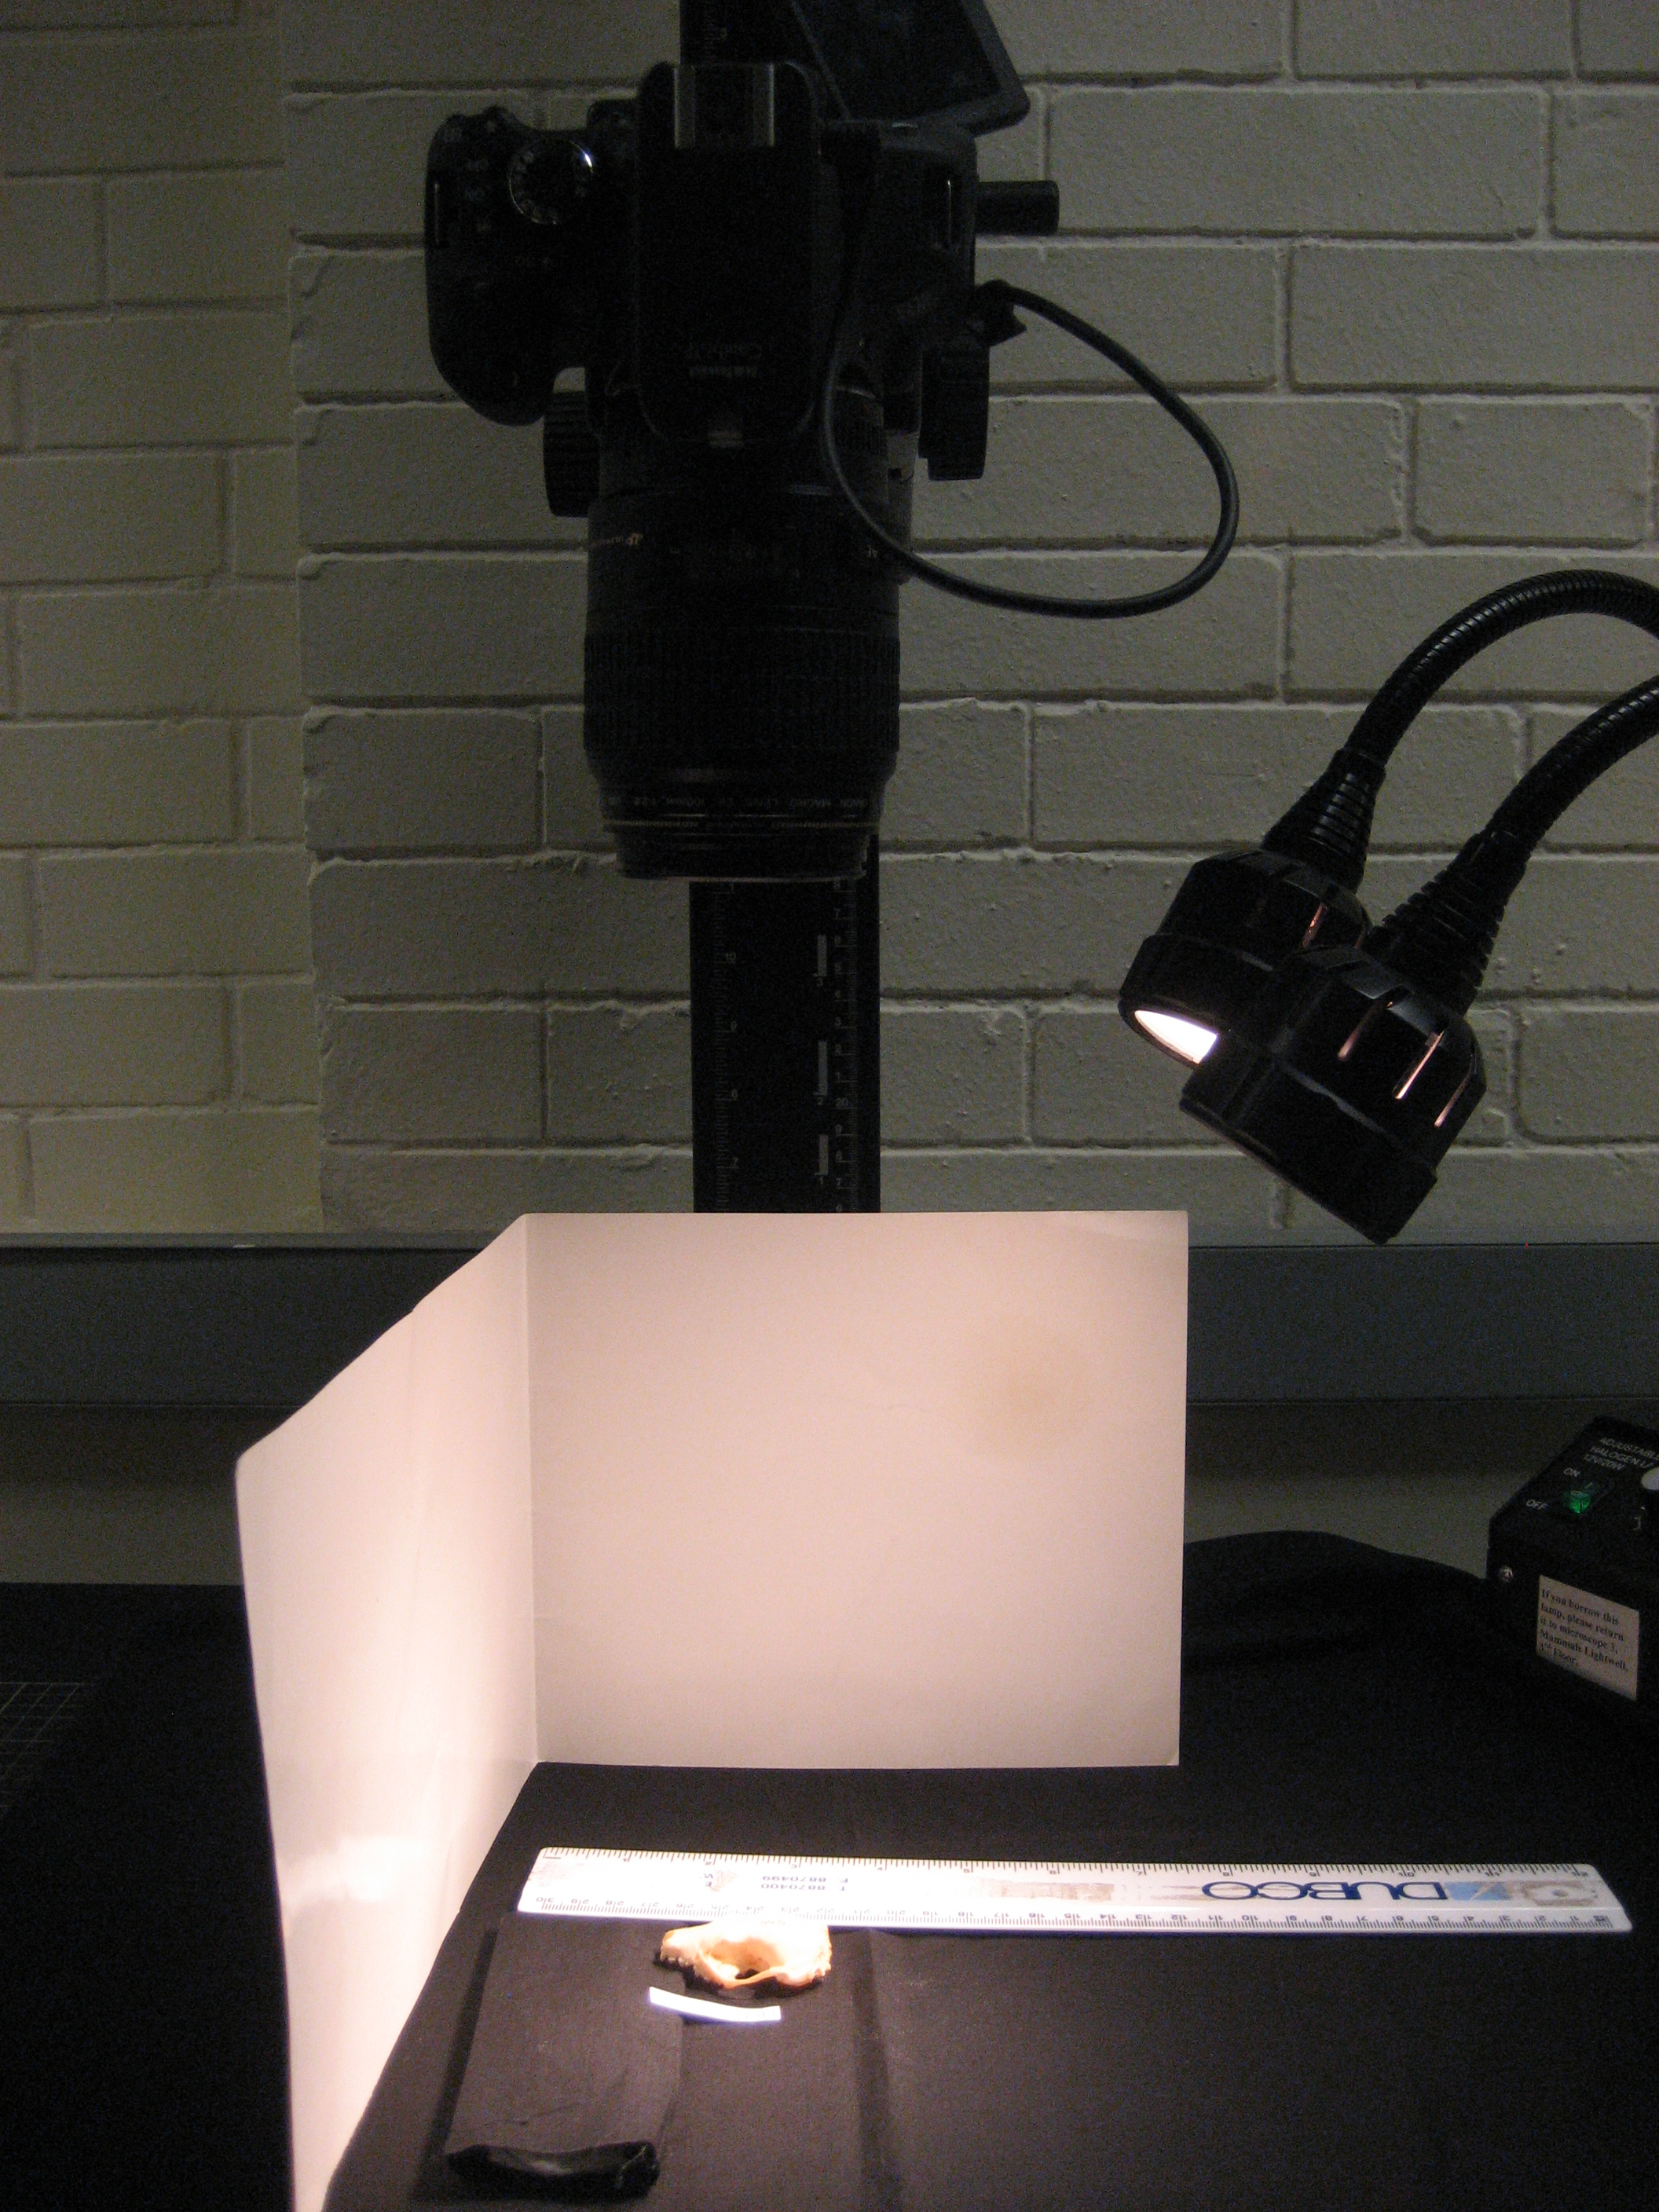
\includegraphics[width=12cm, height=12cm, keepaspectratio=true]{figures/camera.jpg}
    \caption[Photographic set up]%this is what appears in table of contents
    {Photographic set up for taking pictures of skulls. The camera (above centre) is fitted to a copy stand, the light source is directed from the top-left corner of the image and the white card reflects the light back onto the skull. }%this is under the figure
  \label{fig:camera}
  \end{figure}

Photographs were captured and saved in a raw file format. Before using the pictures for morphometric analyses, we converted the raw files to binary (grey scale) images and re-saved them as TIFF files. The black and white pictures were more useful for later analyses since we were not interested in including any colour comparisons and it is easier to see some biological features in binary images. TIFF files were the most appropriate to use for my morphometric analyses as they are uncompressed (in comparison to JPEG) images and therefore there is less chance of any picture distortions which may affect later analyses \citep{HERC2013}.
%----------------------------------------------
%Resampling for minimum number of points
%-----------------------------------------
\section{Determining the number of semilandmarks to use for curves}
When combining landmark and semi-landmark approaches, there is a potential problem of over-sampling the curves (REFS). To determine the number of semilandmark points required to adequately summarise the curves in our data sets,  we followed the method outlined by MacLeod \citeyearpar{MacLeod2012}. 
For each data set we chose a random selection of pictures of specimens which represented the breadth of the morphological data (i.e. specimens from each sub-group of species).  We drew the appropriate curves on the each specimen and over-sampled the number of points on the curves (i.e. resampled the curves so that points were very close together). 
We measured the length of the line and regarded that as the 100\%, true length of that outline. We then re-sampled the curves with decreasing numbers of points and measured the length of the outlines. We calculated the length of the curves resampled with fewere points as a percentage of the total length of the curve. We repeated these calculations for each specimen and then found the average percentage length for each resampled curve across all of the specimens in the test file. We continued this process until we found the minimum number of points that, on average, gave a curve length which was at least a 96\% accurate representatio of the true (over-sampled) curve length.  
We repeated these curve-sampling tests for each analysis (skulls in dorsal/ventral/lateral views and mandibles in lateral view) to determine the minimum number of semilandmark points which would give accurate representations of morphological shape.

%---------------------------------------------------------
%Landmarks and results for ventral and lateral skull views
%---------------------------------------------------------
\section{Additional skull analyses}

%--------------------------------------
\subsection{Landmark placement}

\subsubsection{Skulls: lateral view}
I placed nine landmarks on the lateral pictures (see figure \ref{fig:sklat_landmarks}) and also drew two semilandmark curves between landmarks 7 and 8 to represent the shape of the back of the skull (resampled to 20 semilandmark points) and landmarks 8 and 1 (resampled to 15 semilandmark points) down the midline of the nose to represent the shape of the top of the skull. Table \ref{tab:sklat} describes the definitions for each of the landmark points. 
For specimens that were damaged on their right side we reflected photographs of the left lateral side of the skull so that all pictures would be in the same orientation.

%Sklat diagram and landmarks description
\begin{figure}[H] 
  \centering
  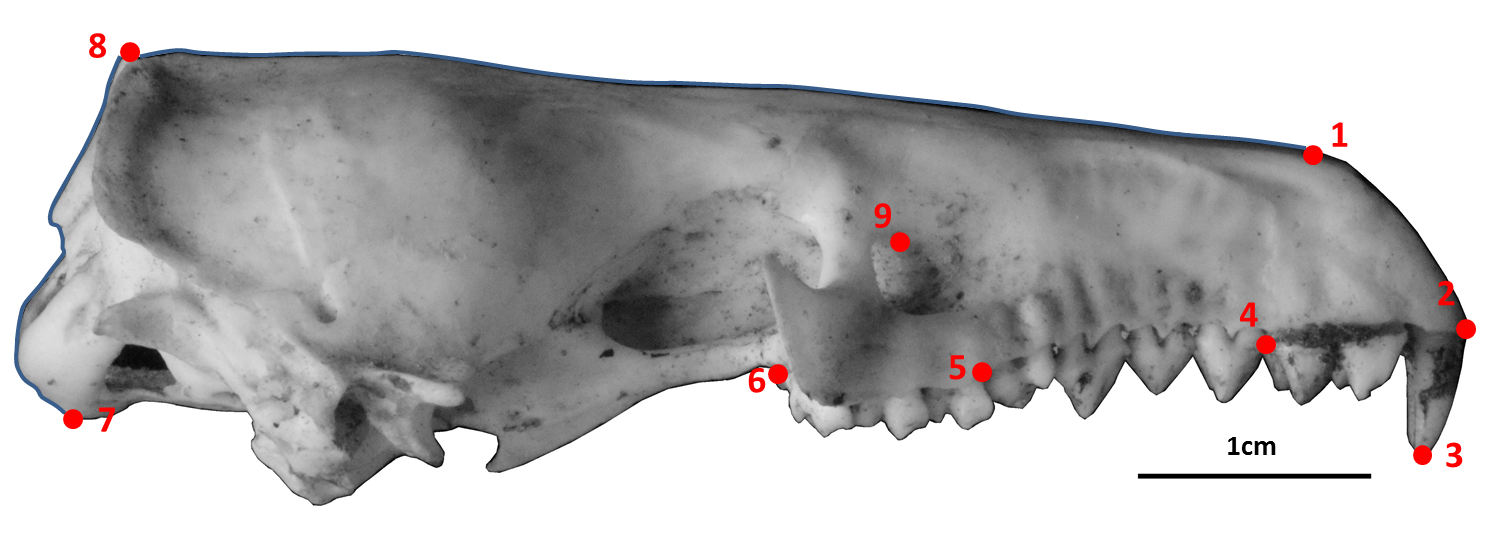
\includegraphics[width=12cm, height=12cm, keepaspectratio=true]
  {figures/sklat_landmarks_pot_vel.png}
    \caption {Landmarks (red) and curve (blue) for the ventral skull pictures, further descriptions in table \ref{tab:sklat}. The specimen is a giant otter shrew tenrec, \textit{Potamogale velox}, NHML 1934.6.16.2}
  \label{fig:sklat_landmarks}
  \end{figure}


% Skulls lateral landmarks
\begin{table}[h]
\caption{Descriptions of the landmarks (points) and curves (semilandmarks) for the skulls in ventral view (see Figure \ref{fig:sklat_landmarks}.} 
%Sklat landmarks
\begin{tabular}[t]{l l}		
\hline
\textbf{Landmark} & \textbf{Description} \\
\hline
%--------------------------------------
1 & Anterior, upper tip of the nasal bone\\
%--------------------------------------
2 & Anterior of the alveolus of the first incisor\\
%--------------------------------------
3 & Lowest point of the first incisor\\
%--------------------------------------
4& Posterior of the alveolus of the last incisor \\
%--------------------------------------
5 & Anterior tip of the alveolus of the first molar\\
%--------------------------------------
6 & Posterior tip of the alveolus of the last molar\\
%--------------------------------------
7 & Lowest point of the basi-occipital (base of the back of the skull)\\
%--------------------------------------
8 & Highest point of the braincase\\
%--------------------------------------
9 & Highest point of the infraorbital foramen\\
%--------------------------------------
\hline
\textbf{Curve A} & Between points 7 and 8  \\
(20 points)& Back of the skull from the lowest to highest points\\
%------------------------------------------------------------
\textbf{Curve B} & Between points 8 and 1  \\
(15 points)&From the highest point of the braincase to the front of the nasal \\
%------------------------------------------------------------
\hline
\end{tabular}
\label{tab:sklat}
\end{table}
%-------------------------------------------

\subsubsection{Skulls: ventral view}
Most of the landmarks in this view are concentrated around the dentition and palate of the animals. We placed 13 landmarks and drew one outline curve (resampled to 60 semilandmark points) around the back of the skulls between landmarks 12 and 13 (figure \ref{fig:skvent_landmarks}). The high variability of the species’ basi-cranial region and difficulties associated with identifying developmentally or functionally homologous points precluded designation of additional landmarks towards the back of the skulls. Table \ref{tab:skvent} outlines the descriptions of the landmarks we placed on the ventral pictures.


%Skvent diagram and landmarks description
\begin{figure}[H] 
  \centering
  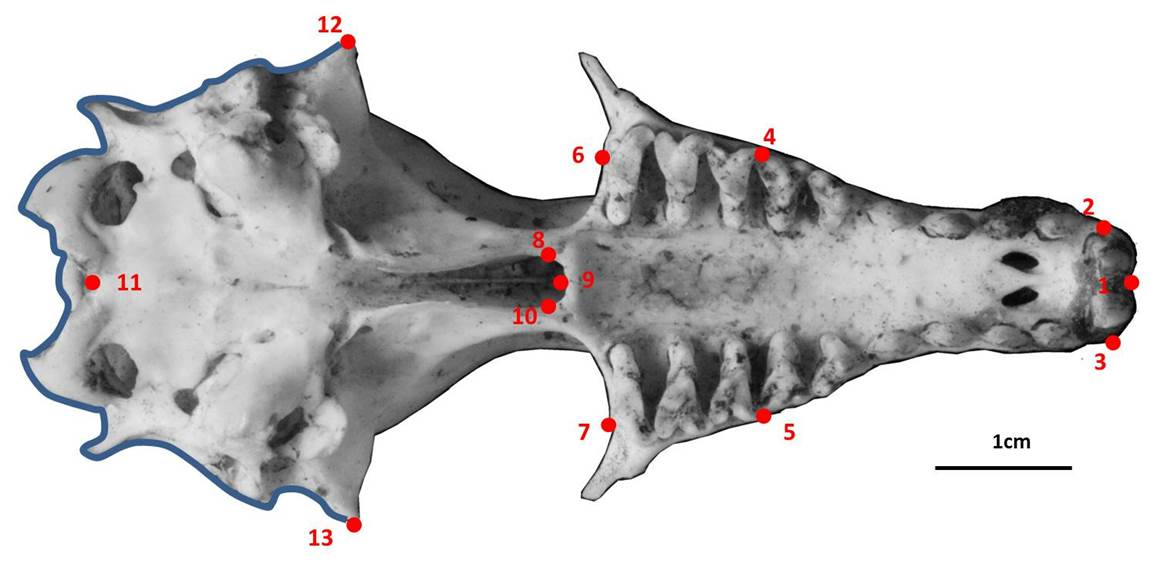
\includegraphics[width=12cm, height=12cm, keepaspectratio=true]
  {figures/skvent_landmarks_pot_vel.jpg}
    \caption {Landmarks (red) and curve (blue) for the ventral skull pictures, further descriptions in table \ref{tab:skvent}. The specimen is a giant otter shrew tenrec, \textit{Potamogale velox}, NHML 1934.6.16.2}
  \label{fig:skvent_landmarks}
  \end{figure}


% Skulls ventral landmarks
\begin{table}[h]
\caption{Descriptions of the landmarks (points) and curves (semilandmarks) for the skulls in ventral view (see Figure \ref{fig:skvent_landmarks}.} 
%SkVent landmarks
\begin{tabular}[t]{l l}		
\hline
\textbf{Landmark} & \textbf{Description} \\
\hline
%--------------------------------------
1 & Anterior point of the palate\\
%--------------------------------------
2 + 3 & Posterior, lateral extremity of the right (2) and left(3) incisor\\
%--------------------------------------
4 + 5 & Anterior, outer point of the first molar on the right (4) and left (5)\\
%--------------------------------------
6 + 7 & Posterior, outermost point of the molar surface on the right (6) and left (7) \\
%--------------------------------------
8 & Widest point of the curve of the palatine on the right side\\
%--------------------------------------
9 & Posterior point of the palatine in the midline\\
%--------------------------------------
10 & Widest point of the curve of the palatine on the left side\\
%--------------------------------------
11 & Anterior of the occipital foramen in the midline\\
%--------------------------------------
12 + 13 & Widest (extreme lateral) point of the braincase on the right (12) and left (13)\\
%--------------------------------------
Curve* & Outline of the back of the skull (between landmarks 12 and 13), 60 points \\
%------------------------------------------------------------
\hline
&*NB: This curve doesn't necessarily trace homologous features because of the \\ 
& variation in the position of the foramen magnum.
\end{tabular}
\label{tab:skvent}
\end{table}

%--------------------------------------------
\subsection{Disparity analysis}


We compared observed disparity to calculations of disparity from BM simulations of shape data (1,000 simulations on each of 101 phylogenies). Our analyses for both the lateral skulls (table \ref{tab:sklat_sims}) and ventral skulls (table \ref{tab:skvent_sims}) supported our findings for the dorsal skulls (table \ref{tab:skdors_sims}) and mandibles (table \ref{tab:mands_sims}): the true (observed) disparity values were significantly lower than expected compared to the distribution of simulated values. The same patterns were true in each of our five disparity metrics; four of which were based on the PC scores of each species (sum and product of range and variance) and disparity calculated as the sum of squared distances between species pairs \citep{Zelditch2012}. 

%--------------------------------------
%Tables of simulation results

\begin{table}[H]				

\centering
\caption{Comparison of observed and simulated disparity measures for the dorsal skulls analysis; observed (true) disparity measures, minimum simulated value (sim.min), maximum simulated value (sim.max), standard deviation of the simulated values (sdev.sim) and p value comparing the observed disparity measures to the distribution of simulated values)}

%Sklat simulation results (disp in the script file)

\begin{tabular}[t]{l l l l l l }		%l left aligns p gives defined col width for long entries
\hline
%\
\textbf{Disparity metric} & \textbf{Observed} & \textbf{Sim.min} & \textbf{Sim.max} & \textbf{Sdev.sim} & \textbf{p value} \\
%\multicolumn{6}{c}{}\\	% empty line below the column headers
\hline
Sum of Variance & 0.0026 & 23768.99 & 352047.7 & 21020.33 &  0\\
%---------------------------------------
Product of Variance	& 0.00014 &	1145.99 &	62118.9 &	1590.39 &	0\\
%-------------------------------
Sum of Ranges &	0.56 &	1464.11 &	3090.03 & 	167.77 & 0 \\
%-------------------------------------
Product of Ranges & 0.05 &	141.0053 &	877.23 &	45.29 &	0\\
%-------------------------------------
ZelditchMD & 0.003 & 30629.96 &	422263.07 &	28276.87 &	0\\

\hline
\end{tabular}
\label{tab:skdors_sims} 
\end{table}


\begin{table}[H]				

\centering
\caption{Comparison of observed and simulated disparity measures for the mandibles analysis; observed (true) disparity measures, minimum simulated value (sim.min), maximum simulated value (sim.max), standard deviation of the simulated values (sdev.sim) and p value comparing the observed disparity measures to the distribution of simulated values)}

%Mandibles simulation results (disp in the script file)

\begin{tabular}[t]{l l l l l l }		%l left aligns p gives defined col width for long entries
\hline
\textbf{Disparity metric} & \textbf{Observed} & \textbf{Sim.min} & \textbf{Sim.max} & \textbf{Sdev.sim} & \textbf{p value} \\
\hline
Sum of Variance & 0.0032 & 23459.28 & 286827.19 & 20915.32 &	0\\
Product of Variance	& 0.000189 & 1173.95 &	286827.19 &	3346.28 & 0\\
Sum of Ranges &	0.676 &	1212.44 &	2996.77 &	170.86 & 0 \\
Product of Ranges & 0.0639 & 151.54 & 1520.68 &	60.51 &	0\\
\hline
\end{tabular}
\label{tab:mands_sims}
\end{table}


\begin{table}[H]				
\centering
\caption{Comparison of observed and simulated disparity measures for the lateral skulls analysis; observed (true) disparity measures, minimum simulated value (sim.min), maximum simulated value (sim.max), standard deviation of the simulated values (sdev.sim) and p value comparing the observed disparity measures to the distribution of simulated values.)}

%Sklat simulation results (disp in the script file)

\begin{tabular}[t]{l l l l l l }		%l left aligns p gives defined col width for long entries
\hline
%\
\textbf{Disparity metric} & \textbf{Observed} & \textbf{Sim.min} & \textbf{Sim.max} & \textbf{Sdev.sim} & \textbf{p value} \\
%\multicolumn{6}{c}{}\\	% empty line below the column headers
\hline
Sum of Variance & 0.0026 & 23768.99 & 352047.7 & 21020.33 &  0\\
%---------------------------------------
Product of Variance	& 0.00014 &	1145.99 &	62118.9 &	1590.39 &	0\\
%-------------------------------
Sum of Ranges &	0.56 &	1464.11 &	3090.03 & 	167.77 & 0 \\
%-------------------------------------
Product of Ranges & 0.05 &	141.0053 &	877.23 &	45.29 &	0\\
%-------------------------------------
ZelditchMD & 0.003 & 30629.96 &	422263.07 &	28276.87 &	0\\

\hline
\end{tabular}
\label{tab:sklat_sims} 
\end{table}

\begin{table}[H]				

\centering
\caption{Comparison of observed and simulated disparity measures for the ventral skulls analysis; observed (true) disparity measures, minimum simulated value (sim.min), maximum simulated value (sim.max), standard deviation of the simulated values (sdev.sim) and p value comparing the observed disparity measures to the distribution of simulated values.)}

%SkVent simulation results (disp in the script file)

\begin{tabular}[t]{l l l l l l }		%l left aligns p gives defined col width for long entries
\hline
%\
\textbf{Disparity metric} & \textbf{Observed} & \textbf{Sim.min} & \textbf{Sim.max} & \textbf{Sdev.sim} & \textbf{p value} \\
%\multicolumn{6}{c}{}\\	% empty line below the column headers
\hline
Sum of Variance & 0.003 &	23298.34 &	299844.9 &	21100.88 &	0\\
%---------------------------------------
Product of Variance	& 0.00013 &	1223.94 & 54239.63 &	1596.207 &	0\\
%-------------------------------
Sum of Ranges &	0.63 &	1527.62 &	3014.34 &	167.88 &	0 \\
%-------------------------------------
Product of Ranges & 0.05 &	144.65 & 888.83 &	45.43 &	0\\
%-------------------------------------
ZelditchMD & 0.003 & 29507.82 &	392346.5 &	26782.22 &	0
\\

\hline
\end{tabular}
\label{tab:skvent_sims} 
\end{table}

%----------------------------------------------------------

Figures  \ref{fig:sklatPCA} and \ref{fig:skventPCA} depict the morphospace plots derived from our principal components analyses of average Procrustes-superimposed shape coordinates for each species in our lateral and ventral skull data respectively. We used the principal components axes which accounted for 95\% of the cumulative variation (n = X axes for the lateral skulls analysis and n = X axes for the ventral skulls analysis) to calculate the disparity of each family. 

In the analysis of skulls in lateral view, tenrecs had higher disparity than golden moles for all of the five metrics and they occupy a significantly different area of morphospace (npMANOVA, F=75.07, R$^{2}$ = 0.65,  p =0.001, figure \ref{fig:sklatPCA}).  
%**********NB: I've phrased it like this because I'm not sure whether the npMANOVA is testing morphospace occupation in general or disparity specifically


\begin{figure}[H]
\centering
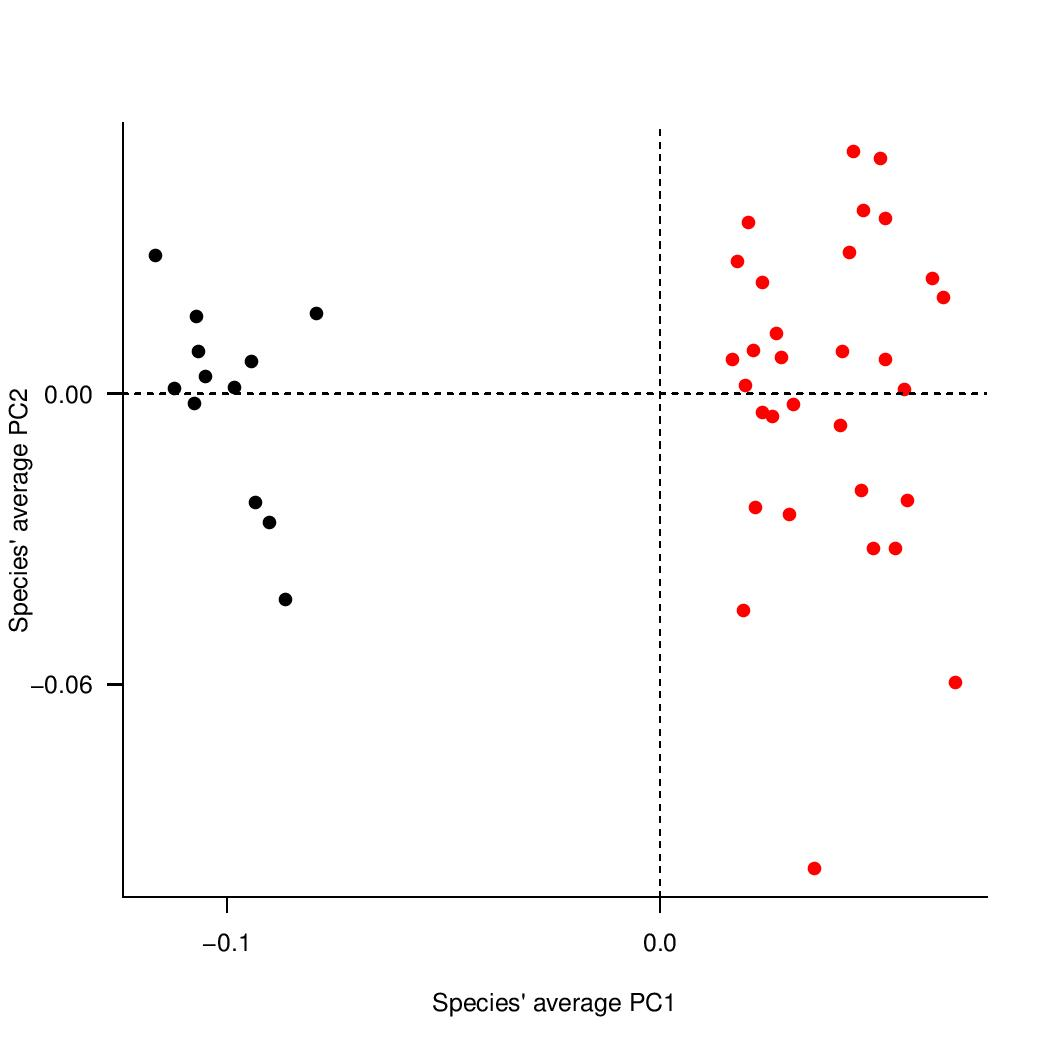
\includegraphics[width=12cm, height=12cm, keepaspectratio=true]
{figures/sklat_tenrec+gmole_PCA.jpg}
\caption{Principal components plot of the lateral skulls' morphospace occupied by tenrecs (red, n=31) and golden moles (black, n=12). Axes are PC1 and PC2 of the average scores from a PCA analysis of mean Procrustes shape coordinates for each species. }
\label{fig:sklatPCA}
\end{figure}


%--------------------------------------------------------
In contrast, in the analysis of skulls in ventral view, tenrecs had higher disparity than golden moles in four of the five metrics but not when we calculated disparity as the sum of ranges.
%*********** Remember I need to put in the disp tables here
The two families occupy significantly different areas of morphospace (npMANOVA, F=100.74, r$^{2}$ = 0.71, p=0.001) but sensitivity analyses indicate that these differences could be artefacts of variation in sample size (section X below).


\begin{figure}[H]
\centering
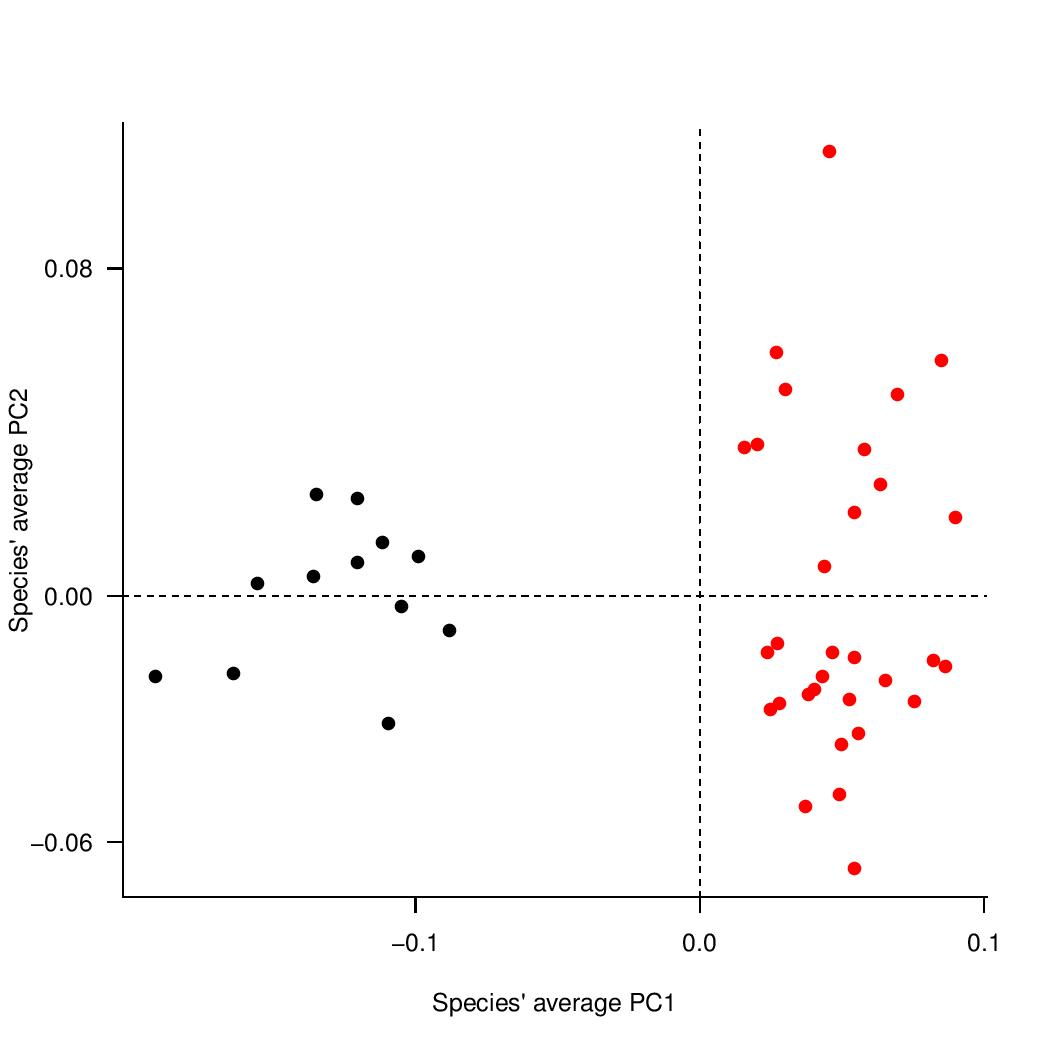
\includegraphics[width=12cm, height=12cm, keepaspectratio=true]
{figures/skvent_tenrec+gmole_PCA.jpg}
\caption{Principal components plot of the lateral skulls' morphospace occupied by tenrecs (red, n=31) and golden moles (black, n=12). Axes are PC1 and PC2 of the average scores from a PCA analysis of mean Procrustes shape coordinates for each species. }
\label{fig:skventPCA}
\end{figure}


%---------------------------------------------------------
%Rarefaction methods and results
%---------------------------------------------------------
\section{Sensitivity analyses}
\subsection{Sample size}

Our calculations of disparity in tenrecs and golden moles are based on the amount of morphospace which is occupied by each group; families which occupy larger areas of morphospace are considered to have higher morphological disparity. However, larger groups might be expected to occupy greater areas of morphospace just because they are represented by more species. We compared a sample of 31 species of tenrec to 12 species of golden moles. Therefore, we used rarefaction analyses to test whether differences in morphospace occupation between the two groups were merely artefacts of variation in sample size.

For each data set (skulls dorsal/ventral/lateral and mandibles) we re-sampled the shape data (average shape for each species) without replacement and repeated the resampling 100 times for each iteration. For tenrecs and golden moles we re-sampled from two to n-1 species i.e. 100 samples of 2 species, 3 species, 4 species etc. We calculated disparity metrics (sum and product of variance and ranges) for each re-sampled iteration and took the average calculated value for that metric and iteration (e.g. average sum of variance from 100 sets of 2 re-sampled species). We used bootstapping (1000 iterations) to calculate 95\% confidence intervals for each sample size. We plotted the mean values and confidence intervals against sample size to depict the expected change in disparity. 

Separate discussion of each data set

%****************************************
%NB: I need to re-create these rarefaction pictures to make them nicer; the confidence intervals are too fuzzy
\begin{figure}[H] 
  \centering
  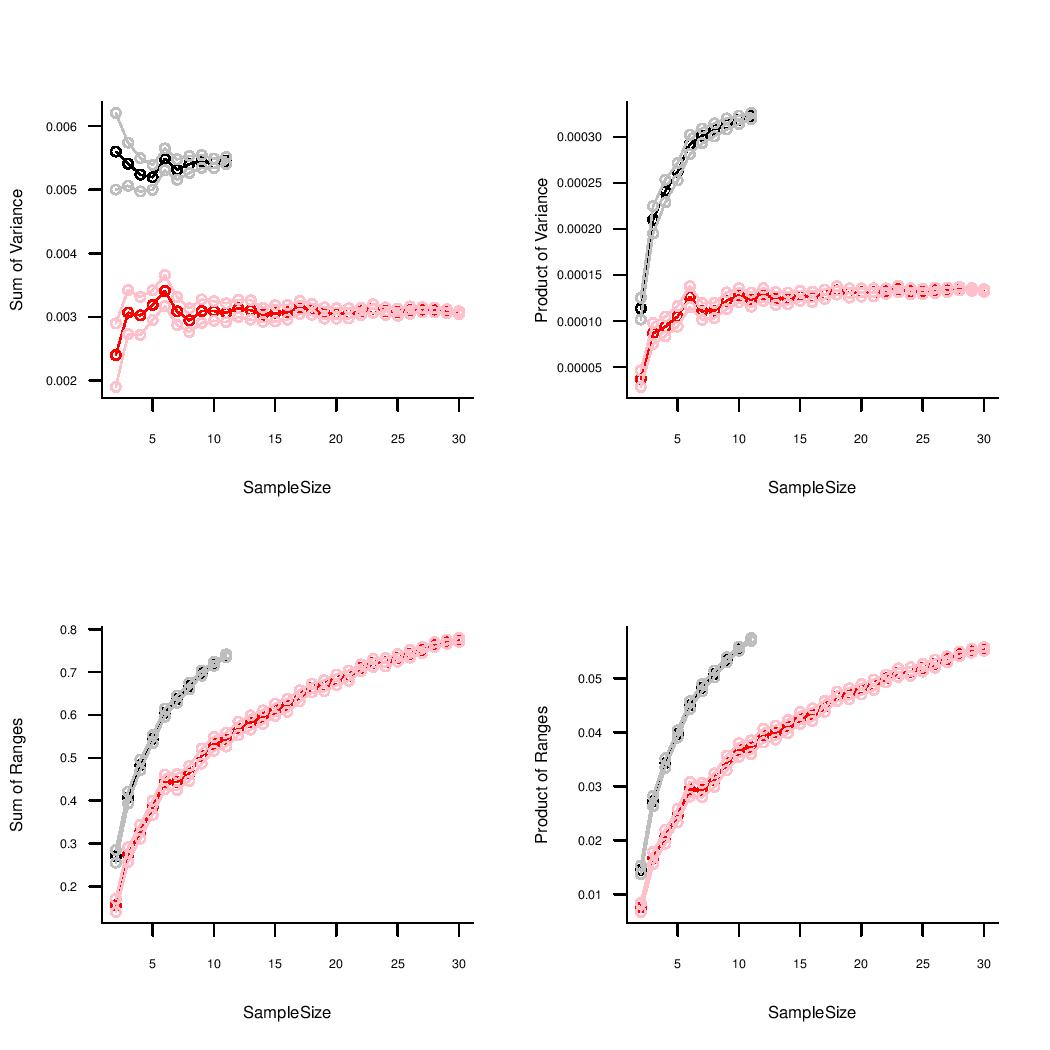
\includegraphics{figures/mands_trc+gmole_PCrarefaction.jpg}
    \caption
    {Rarefaction profiles of disparity metrics for mandibles}%this is under the figure
  \label{fig:mands.rarefaction}
  \end{figure}
%*********************************************     
%---------------------------------------------------------
%Simulation results for non-Microgale tenrecs
%---------------------------------------------------------
\subsection{Comparison of non-\textit{Microgale} tenrecs}


%---------------------------------------------------------
%Table of museum accession numbers
%---------------------------------------------------------
\section{Museum specimens}
%I need to fix the position of the caption
% Table generated by Excel2LaTeX from sheet 'Tenrec_Gmole_skulls_taxonomy'

%\documentclass[12pt]{article}
%\usepackage{longtable}
%\usepackage[margin ={1cm, 1cm, 1cm, 1cm, 1cm}]{geometry}
%\pagenumbering{}
%\begin{document}

%\begin{centre}
\begin{longtable}{|l|l|l|l|l|}

  \caption{Museum accession numbers and taxonomic identification for all skull specimens. AMNH (American Museum of Natural History), FMNH (Field Museum of Natural History), MCZ (Museum of Comparative Zoology, Harvard), NHML (Natural History Museum London), SI (Smithsonian Institute)}{l}\\
  \hline 

\textbf{Specimen ID} & \textbf{Order} & \textbf{Family} & \textbf{Genus} & \textbf{Species} \\
\hline
\endfirsthead

\multicolumn {5} {l}
{{\bfseries \tablename\ \thetable\ --\textit{Continues from previous page}}}\\
  \hline
  \textbf{SpecID} & \textbf{Order} & \textbf{Family} & \textbf{Genus} & \textbf{Species} \\
  \hline
\endhead

\hline \multicolumn{5}{|r|}{\textit{Continued on next page}} \\ 
\hline
\endfoot


\hline 
\endlastfoot

    AMNH\_161526 & Afrosoricida & Chrysochloridae & Chlorotalpa & duthieae \\
    AMNH\_161527 & Afrosoricida & Chrysochloridae & Chlorotalpa & duthieae \\
    AMNH\_161559 & Afrosoricida & Chrysochloridae & Eremitalpa & granti \\
    AMNH\_161571 & Afrosoricida & Chrysochloridae & Eremitalpa & granti \\
    AMNH\_167961 & Afrosoricida & Chrysochloridae & Chrysochloris & asiatica \\
    AMNH\_180911 & Afrosoricida & Chrysochloridae & Chrysochloris & stuhlmanni \\
    AMNH\_180912 & Afrosoricida & Chrysochloridae & Chrysochloris & stuhlmanni \\
    AMNH\_212938 & Afrosoricida & Tenrecidae & Hemicentetes & semispinosus \\
    AMNH\_274982 & Afrosoricida & Tenrecidae & Microgale & jobihely \\
    AMNH\_274986 & Afrosoricida & Tenrecidae & Microgale & jobihely \\
    AMNH\_274987 & Afrosoricida & Tenrecidae & Microgale & jobihely \\
    AMNH\_274988 & Afrosoricida & Tenrecidae & Microgale & jobihely \\
    AMNH\_274989 & Afrosoricida & Tenrecidae & Microgale & jobihely \\
    AMNH\_275041 & Afrosoricida & Tenrecidae & Microgale & soricoides \\
    AMNH\_275088 & Afrosoricida & Tenrecidae & Microgale & drouhardi \\
    AMNH\_275089 & Afrosoricida & Tenrecidae & Microgale & drouhardi \\
    AMNH\_275090 & Afrosoricida & Tenrecidae & Microgale & drouhardi \\
    AMNH\_275092 & Afrosoricida & Tenrecidae & Microgale & drouhardi \\
    AMNH\_275095 & Afrosoricida & Tenrecidae & Microgale & drouhardi \\
    AMNH\_275133 & Afrosoricida & Tenrecidae & Microgale & fotsifotsy \\
    AMNH\_275134 & Afrosoricida & Tenrecidae & Microgale & gymnorhyncha \\
    AMNH\_275135 & Afrosoricida & Tenrecidae & Microgale & gymnorhyncha \\
    AMNH\_275136 & Afrosoricida & Tenrecidae & Microgale & gymnorhyncha \\
    AMNH\_275137 & Afrosoricida & Tenrecidae & Microgale & gymnorhyncha \\
    AMNH\_275138 & Afrosoricida & Tenrecidae & Microgale & gymnorhyncha \\
    AMNH\_275141 & Afrosoricida & Tenrecidae & Microgale & longicaudata \\
    AMNH\_275142 & Afrosoricida & Tenrecidae & Microgale & longicaudata \\
    AMNH\_275143 & Afrosoricida & Tenrecidae & Microgale & longicaudata \\
    AMNH\_275148 & Afrosoricida & Tenrecidae & Microgale & longicaudata \\
    AMNH\_275149 & Afrosoricida & Tenrecidae & Microgale & longicaudata \\
    AMNH\_275157 & Afrosoricida & Tenrecidae & Microgale & parvula \\
    AMNH\_275158 & Afrosoricida & Tenrecidae & Microgale & soricoides \\
    AMNH\_275160 & Afrosoricida & Tenrecidae & Microgale & soricoides \\
    AMNH\_275162 & Afrosoricida & Tenrecidae & Microgale & soricoides \\
    AMNH\_275163 & Afrosoricida & Tenrecidae & Microgale & soricoides \\
    AMNH\_275189 & Afrosoricida & Tenrecidae & Oryzorictes & hova \\
    AMNH\_275190 & Afrosoricida & Tenrecidae & Oryzorictes & hova \\
    AMNH\_275191 & Afrosoricida & Tenrecidae & Oryzorictes & hova \\
    AMNH\_275250 & Afrosoricida & Tenrecidae & Microgale & brevicaudata \\
    AMNH\_275251 & Afrosoricida & Tenrecidae & Microgale & brevicaudata \\
    AMNH\_275253 & Afrosoricida & Tenrecidae & Microgale & brevicaudata \\
    AMNH\_275254 & Afrosoricida & Tenrecidae & Microgale & brevicaudata \\
    AMNH\_275255 & Afrosoricida & Tenrecidae & Microgale & brevicaudata \\
    AMNH\_275281 & Afrosoricida & Tenrecidae & Microgale & fotsifotsy \\
    AMNH\_275282 & Afrosoricida & Tenrecidae & Microgale & fotsifotsy \\
    AMNH\_275283 & Afrosoricida & Tenrecidae & Microgale & fotsifotsy \\
    AMNH\_275298 & Afrosoricida & Tenrecidae & Microgale & taiva \\
    AMNH\_275299 & Afrosoricida & Tenrecidae & Microgale & taiva \\
    AMNH\_275300 & Afrosoricida & Tenrecidae & Microgale & taiva \\
    AMNH\_275301 & Afrosoricida & Tenrecidae & Microgale & taiva \\
    AMNH\_275360 & Afrosoricida & Tenrecidae & Oryzorictes & hova \\
    AMNH\_275364 & Afrosoricida & Tenrecidae & Microgale & parvula \\
    AMNH\_275365 & Afrosoricida & Tenrecidae & Microgale & parvula \\
    AMNH\_275368 & Afrosoricida & Tenrecidae & Microgale & parvula \\
    AMNH\_31243 & Afrosoricida & Tenrecidae & Oryzorictes & tetradactylus \\
    AMNH\_31257 & Afrosoricida & Tenrecidae & Oryzorictes & tetradactylus \\
    AMNH\_31270 & Afrosoricida & Tenrecidae & Echinops & telfairi \\
    AMNH\_34647 & Afrosoricida & Chrysochloridae & Chrysospalax & trevelyani \\
    AMNH\_51324 & Afrosoricida & Tenrecidae & Potamogale & velox \\
    AMNH\_51327 & Afrosoricida & Tenrecidae & Potamogale & velox \\
    AMNH\_54365 & Afrosoricida & Chrysochloridae & Chrysospalax & trevelyani \\
    AMNH\_82399 & Afrosoricida & Chrysochloridae & Chrysochloris & stuhlmanni \\
    AMNH\_89040 & Afrosoricida & Chrysochloridae & Chrysospalax & trevelyani \\
    AMNH\_89046 & Afrosoricida & Chrysochloridae & Cryptochloris & wintoni \\
    FMNH\_156226 & Afrosoricida & Tenrecidae & Oryzorictes & tetradactylus \\
    FMNH\_159672 & Afrosoricida & Tenrecidae & Microgale & monticola \\
    FMNH\_159673 & Afrosoricida & Tenrecidae & Microgale & monticola \\
    FMNH\_159674 & Afrosoricida & Tenrecidae & Microgale & monticola \\
    FMNH\_159675 & Afrosoricida & Tenrecidae & Microgale & monticola \\
    FMNH\_159676 & Afrosoricida & Tenrecidae & Microgale & monticola \\
    FMNH\_162893 & Afrosoricida & Tenrecidae & Micropotamogale & lamottei \\
    FMNH\_166040 & Afrosoricida & Tenrecidae & Microgale & pusilla \\
    FMNH\_166111 & Afrosoricida & Tenrecidae & Microgale & gracilis \\
    FMNH\_166112 & Afrosoricida & Tenrecidae & Microgale & gracilis \\
    FMNH\_166113 & Afrosoricida & Tenrecidae & Microgale & gracilis \\
    FMNH\_166145 & Afrosoricida & Tenrecidae & Microgale & gracilis \\
    FMNH\_167427 & Afrosoricida & Tenrecidae & Microgale & dryas \\
    FMNH\_167621 & Afrosoricida & Tenrecidae & Microgale & pusilla \\
    FMNH\_176203 & Afrosoricida & Tenrecidae & Geogale & aurita \\
    FMNH\_176204 & Afrosoricida & Tenrecidae & Geogale & aurita \\
    FMNH\_176211 & Afrosoricida & Tenrecidae & Geogale & aurita \\
    FMNH\_176385 & Afrosoricida & Tenrecidae & Microgale & dryas \\
    FMNH\_176387 & Afrosoricida & Tenrecidae & Microgale & dryas \\
    FMNH\_176389 & Afrosoricida & Tenrecidae & Microgale & dryas \\
    FMNH\_176395 & Afrosoricida & Tenrecidae & Microgale & dryas \\
    FMNH\_209199 & Afrosoricida & Tenrecidae & Microgale & grandidieri \\
    FMNH\_209200 & Afrosoricida & Tenrecidae & Microgale & grandidieri \\
    FMNH\_209201 & Afrosoricida & Tenrecidae & Microgale & grandidieri \\
    FMNH\_209202 & Afrosoricida & Tenrecidae & Microgale & grandidieri \\
    FMNH\_209203 & Afrosoricida & Tenrecidae & Microgale & grandidieri \\
    FMNH\_53073 & Afrosoricida & Chrysochloridae & Amblysomus & corriae \\
    FMNH\_72831 & Afrosoricida & Tenrecidae & Potamogale & velox \\
    FMNH\_81731 & Afrosoricida & Chrysochloridae & Calcochloris & leucorhinus \\
    FMNH\_83540 & Afrosoricida & Chrysochloridae & Calcochloris & leucorhinus \\
    MCZ\_23373 & Afrosoricida & Chrysochloridae & Chrysochloris & stuhlmanni \\
    MCZ\_45021 & Afrosoricida & Tenrecidae & Oryzorictes & tetradactylus \\
    MCZ\_45022 & Afrosoricida & Tenrecidae & Oryzorictes & tetradactylus \\
    MCZ\_45033 & Afrosoricida & Tenrecidae & Microgale & pusilla \\
    MCZ\_45050 & Afrosoricida & Tenrecidae & Limnogale & mergulus \\
    MCZ\_45450 & Afrosoricida & Tenrecidae & Geogale & aurita \\
    MCZ\_46274 & Afrosoricida & Tenrecidae & Geogale & aurita \\
    NHML\_1870.3.10.15\_1527.a & Afrosoricida & Tenrecidae & Setifer & setosus \\
    NHML\_1934.6.16.2 & Afrosoricida & Tenrecidae & Potamogale & velox \\
    NHML\_1961.6.2.3 & Afrosoricida & Chrysochloridae & Chrysospalax & trevelyani \\
    NHML\_3.1.1.1 & Afrosoricida & Tenrecidae & Geogale & aurita \\
    NHML\_3.6.2.10 & Afrosoricida & Chrysochloridae & Amblysomus & hottentotus \\
    NHML\_3509 & Afrosoricida & Tenrecidae & Tenrec & ecaudatus \\
    NHML\_67.213 & Afrosoricida & Tenrecidae & Micropotamogale & ruwenzorii \\
    NHML\_73.170 & Afrosoricida & Tenrecidae & Micropotamogale & lamottei \\
    NHML\_74.668 & Afrosoricida & Chrysochloridae & Chrysochloris & sp. \\
    NHML\_75.2223 & Afrosoricida & Tenrecidae & Microgale & cowani \\
    NHML\_82.3.1.11 & Afrosoricida & Tenrecidae & Hemicentetes & nigriceps \\
    SI\_083658 & Afrosoricida & Tenrecidae & Hemicentetes & semispinosus \\
    SI\_154988 & Afrosoricida & Tenrecidae & Microgale & dobsoni \\
    SI\_154989 & Afrosoricida & Tenrecidae & Oryzorictes & tetradactylus \\
    SI\_221420 & Afrosoricida & Chrysochloridae & Chlorotalpa & duthieae \\
    SI\_266897 & Afrosoricida & Tenrecidae & Potamogale & velox \\
    SI\_294497 & Afrosoricida & Tenrecidae & Setifer & setosus \\
    SI\_294504 & Afrosoricida & Tenrecidae & Hemicentetes & semispinosus \\
    SI\_294507 & Afrosoricida & Tenrecidae & Hemicentetes & nigriceps \\
    SI\_294508 & Afrosoricida & Tenrecidae & Hemicentetes & nigriceps \\
    SI\_294510 & Afrosoricida & Tenrecidae & Hemicentetes & nigriceps \\
    SI\_294511 & Afrosoricida & Tenrecidae & Hemicentetes & nigriceps \\
    SI\_294520 & Afrosoricida & Tenrecidae & Microgale & dobsoni \\
    SI\_328604 & Afrosoricida & Tenrecidae & Setifer & setosus \\
    SI\_328605 & Afrosoricida & Tenrecidae & Setifer & setosus \\
    SI\_328614 & Afrosoricida & Tenrecidae & Setifer & setosus \\
    SI\_328616 & Afrosoricida & Tenrecidae & Echinops & telfairi \\
    SI\_328619 & Afrosoricida & Tenrecidae & Echinops & telfairi \\
    SI\_328622 & Afrosoricida & Tenrecidae & Echinops & telfairi \\
    SI\_328624 & Afrosoricida & Tenrecidae & Echinops & telfairi \\
    SI\_328653 & Afrosoricida & Tenrecidae & Microgale & cowani \\
    SI\_328662 & Afrosoricida & Tenrecidae & Microgale & cowani \\
    SI\_328667 & Afrosoricida & Tenrecidae & Microgale & cowani \\
    SI\_328669 & Afrosoricida & Tenrecidae & Microgale & cowani \\
    SI\_328670 & Afrosoricida & Tenrecidae & Microgale & cowani \\
    SI\_328688 & Afrosoricida & Tenrecidae & Microgale & pusilla \\
    SI\_328689 & Afrosoricida & Tenrecidae & Microgale & pusilla \\
    SI\_328690 & Afrosoricida & Tenrecidae & Microgale & pusilla \\
    SI\_328695 & Afrosoricida & Tenrecidae & Microgale & dobsoni \\
    SI\_341621 & Afrosoricida & Tenrecidae & Tenrec & ecaudatus \\
    SI\_341624 & Afrosoricida & Tenrecidae & Tenrec & ecaudatus \\
    SI\_341661 & Afrosoricida & Tenrecidae & Hemicentetes & semispinosus \\
    SI\_341688 & Afrosoricida & Tenrecidae & Hemicentetes & semispinosus \\
    SI\_341689 & Afrosoricida & Tenrecidae & Hemicentetes & semispinosus \\
    SI\_351334 & Afrosoricida & Chrysochloridae & Calcochloris & obtusirostris \\
    SI\_351335 & Afrosoricida & Chrysochloridae & Calcochloris & obtusirostris \\
    SI\_351336 & Afrosoricida & Chrysochloridae & Chrysospalax & villosus \\
    SI\_351955 & Afrosoricida & Chrysochloridae & Calcochloris & obtusirostris \\
    SI\_361482 & Afrosoricida & Tenrecidae & Tenrec & ecaudatus \\
    SI\_365001 & Afrosoricida & Chrysochloridae & Carpitalpa & arendsi \\
    SI\_380484 & Afrosoricida & Chrysochloridae & Amblysomus & hottentotus \\
    SI\_380485 & Afrosoricida & Chrysochloridae & Amblysomus & hottentotus \\
    SI\_381488 & Afrosoricida & Chrysochloridae & Amblysomus & hottentotus \\
    SI\_395676 & Afrosoricida & Tenrecidae & Geogale & aurita \\
    SI\_449177 & Afrosoricida & Tenrecidae & Microgale & taiva \\
    SI\_449179 & Afrosoricida & Tenrecidae & Microgale & gracilis \\
    SI\_449192 & Afrosoricida & Tenrecidae & Microgale & dobsoni \\
    SI\_468315 & Afrosoricida & Chrysochloridae & Chrysochloris & asiatica \\
    SI\_468316 & Afrosoricida & Chrysochloridae & Chrysochloris & asiatica \\
    SI\_468317 & Afrosoricida & Chrysochloridae & Chrysochloris & asiatica \\
    SI\_468318 & Afrosoricida & Chrysochloridae & Eremitalpa & granti \\
    SI\_468319 & Afrosoricida & Chrysochloridae & Cryptochloris & wintoni \\
    SI\_470211 & Afrosoricida & Chrysochloridae & Calcochloris & obtusirostris \\
    SI\_537651 & Afrosoricida & Tenrecidae & Potamogale & velox \\
    SI\_577052 & Afrosoricida & Tenrecidae & Oryzorictes & hova \\
    SI\_577055 & Afrosoricida & Tenrecidae & Microgale & talazaci \\
    SI\_578746 & Afrosoricida & Tenrecidae & Microgale & talazaci \\
    SI\_578747 & Afrosoricida & Tenrecidae & Microgale & talazaci \\
    SI\_578749 & Afrosoricida & Tenrecidae & Microgale & dobsoni \\
    SI\_578753 & Afrosoricida & Tenrecidae & Microgale & principula \\
    SI\_578756 & Afrosoricida & Tenrecidae & Microgale & principula \\
    SI\_578759 & Afrosoricida & Tenrecidae & Microgale & principula \\
    SI\_578760 & Afrosoricida & Tenrecidae & Microgale & principula \\
    SI\_578762 & Afrosoricida & Tenrecidae & Microgale & principula \\
    SI\_578768 & Afrosoricida & Tenrecidae & Microgale & talazaci \\
    SI\_578769 & Afrosoricida & Tenrecidae & Microgale & talazaci \\
    SI\_578772 & Afrosoricida & Tenrecidae & Microgale & thomasi \\
    SI\_578773 & Afrosoricida & Tenrecidae & Microgale & thomasi \\
    SI\_578774 & Afrosoricida & Tenrecidae & Microgale & thomasi \\
    SI\_578775 & Afrosoricida & Tenrecidae & Microgale & thomasi \\
    SI\_578776 & Afrosoricida & Tenrecidae & Microgale & thomasi \\
    SI\_578784 & Afrosoricida & Tenrecidae & Microgale & parvula \\
    SI\_578787 & Afrosoricida & Tenrecidae & Microgale & fotsifotsy \\
    SI\_578789 & Afrosoricida & Tenrecidae & Oryzorictes & sp. \\
    SI\_578791 & Afrosoricida & Tenrecidae & Tenrec & ecaudatus \\
    SI\_578792 & Afrosoricida & Tenrecidae & Tenrec & ecaudatus \\
    SI\_584649 & Afrosoricida & Chrysochloridae & Calcochloris & leucorhinus \\

\end{longtable}
%\end{centre}
%\end{document}

%  \label{tab:sk.taxonomy}%
%\end{table}%

\bibliographystyle{jeb}
\bibliography{Refs_01_05_14_edited}
\end{document}